\documentclass{standalone}
\usepackage{pgfplots}
\usepackage{lmodern}
\pgfplotsset{compat=1.17}

\begin{document}
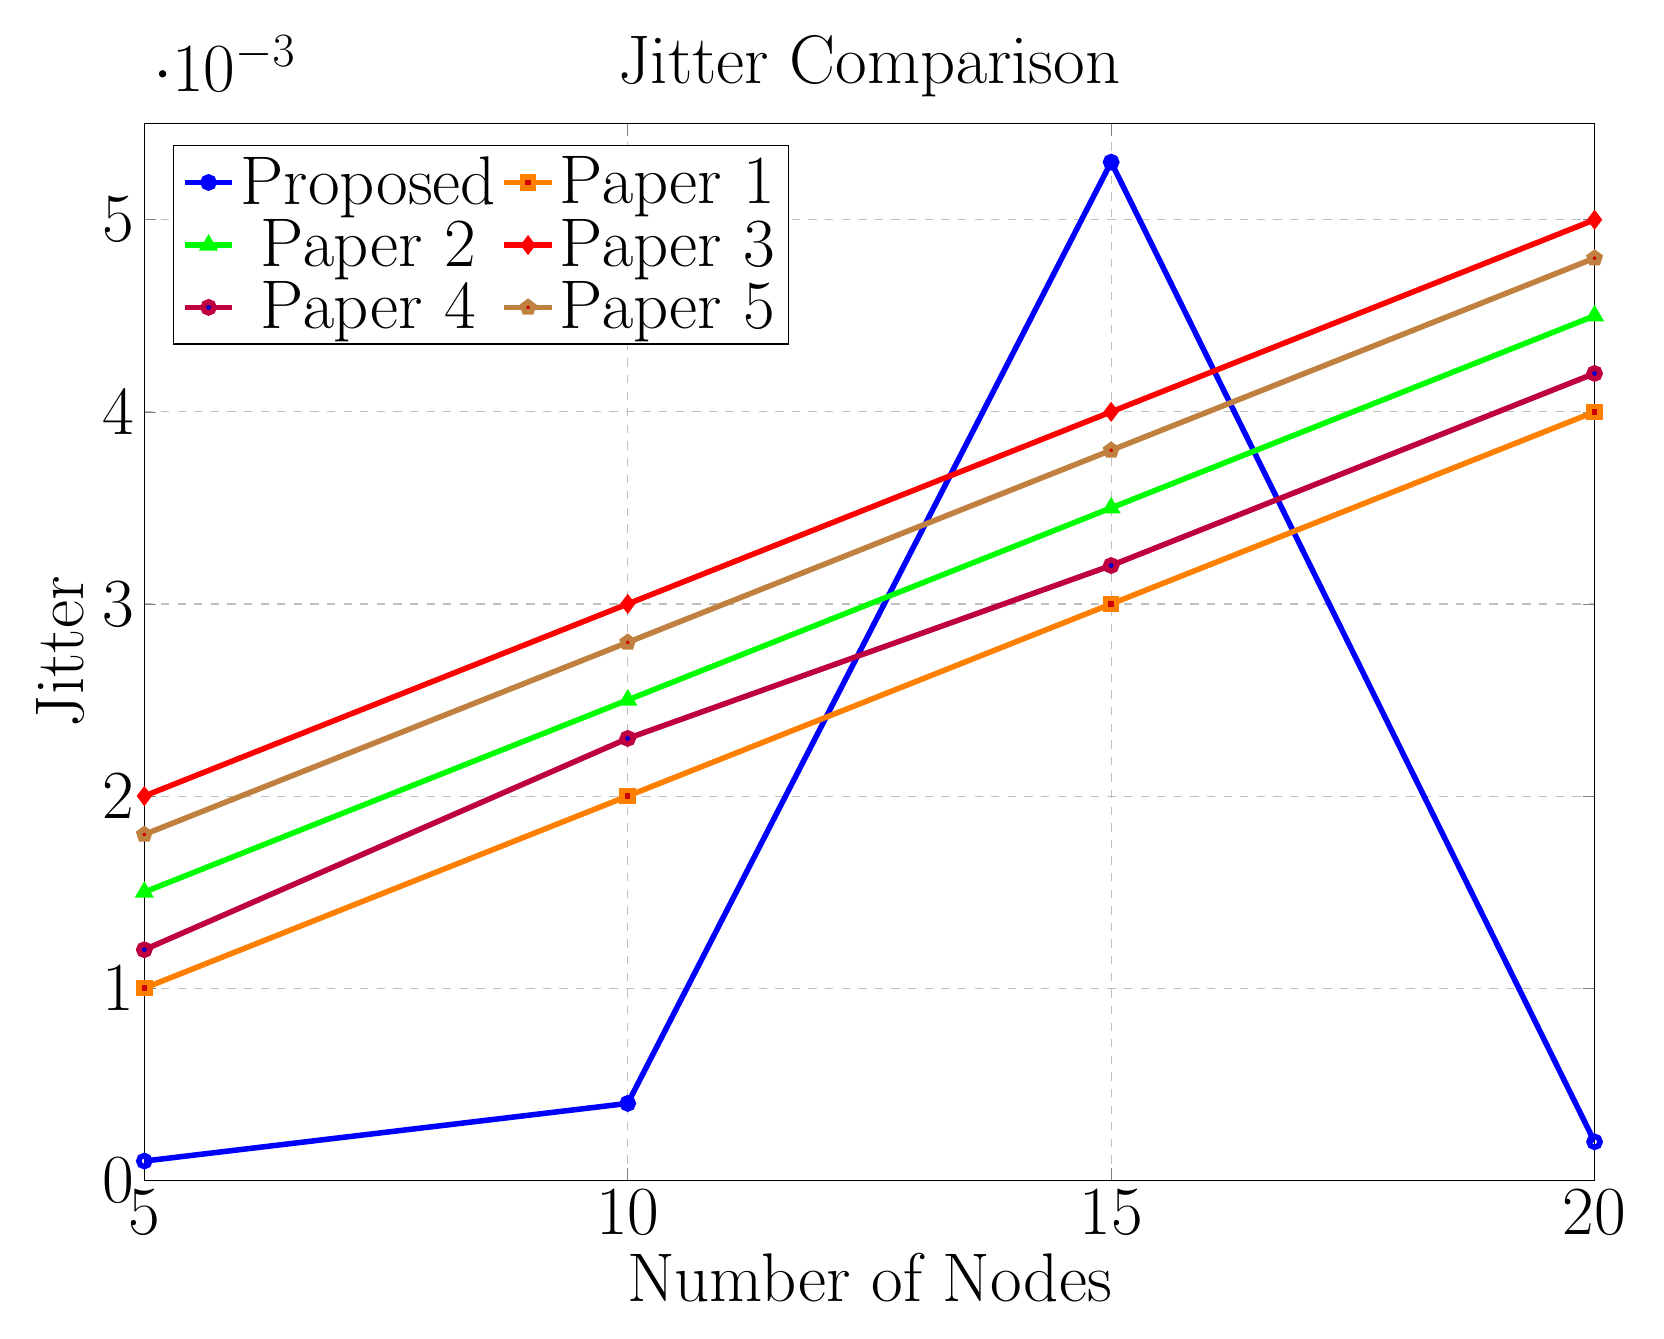
\begin{tikzpicture}
\begin{axis}[
 width=20cm,
 height=15cm,
 tick label style={font=\fontsize{24}{28}\selectfont},
 label style={font=\fontsize{24}{28}\selectfont},
 title style={font=\fontsize{24}{28}\selectfont},
 title={Jitter Comparison},
 xlabel={Number of Nodes},
 ylabel={Jitter},
 xmin=5, xmax=20,
 ymin=0, ymax=0.0055,
 xtick={5,10,15,20},
 ytick={0,0.001,0.002,0.003,0.004,0.005},
 legend columns=2,
 legend style={
 font=\fontsize{24}{28}\selectfont,
 at={(0.02,0.98)},
 anchor=north west,
 draw=black,
 fill=white
 },
 ymajorgrids=true,
 xmajorgrids=true,
 grid style=dashed
]

% Proposed
\addplot+[mark=o,color=blue,line width=2pt] coordinates {
 (5,0.0001)(10,0.0004)(15,0.0053)(20,0.0002)
};

% Paper 1
\addplot+[mark=square*,color=orange,line width=2pt] coordinates {
 (5,0.001)(10,0.002)(15,0.003)(20,0.004)
};

% Paper 2
\addplot+[mark=triangle*,color=green,line width=2pt] coordinates {
 (5,0.0015)(10,0.0025)(15,0.0035)(20,0.0045)
};

% Paper 3
\addplot+[mark=diamond*,color=red,line width=2pt] coordinates {
 (5,0.002)(10,0.003)(15,0.004)(20,0.005)
};

% Paper 4
\addplot+[mark=*,color=purple,line width=2pt] coordinates {
 (5,0.0012)(10,0.0023)(15,0.0032)(20,0.0042)
};

% Paper 5
\addplot+[mark=pentagon*,color=brown,line width=2pt,solid] coordinates {
 (5,0.0018)(10,0.0028)(15,0.0038)(20,0.0048)
};

\legend{Proposed, Paper 1, Paper 2, Paper 3, Paper 4, Paper 5}

\end{axis}
\end{tikzpicture}
\end{document}